\chapter{Introduction}
\label{sec:introduction}

This thesis presents the first observation of the Higgs boson decaying to a pair
of tau leptons ($\Pgt^{+}\Pgt^{-}$) at 13\TeV. It includes two analyses which target different
ways the Higgs boson is produced. The analyses are performed using
13\TeV center-of-mass energy proton-proton collision data from the CERN LHC.
The data is collected by the CMS experiment and corresponds to an integrated
luminosity of 35.9\fbinv. The results here constitutes an important
milestone in the effort to better understand the fundamental properties of nature and
the Higgs boson, one of the fundamental particles of the standard model (SM) of physics.

The standard model of physics is a mathematical framework for explaining
the interactions and behavior of the fundamental particles observed in nature.
It has been built up and defined through the 1950s and 60s culminating in the
theoretical prediction of the existence of a neutral scalar boson, now called the
Higgs boson.
The SM incorporates descriptions of three of the four fundamental forces of nature:
the strong force, the electromagnetic force, and the weak force.
The gravitational force is the one fundamental force not described in the SM. 

The Higgs boson eluded observation by experimental particle physicists
for 40 years after the establishment of its theoretical prediction. 
In 2012, the Higgs boson was discovered 
by the CMS and ATLAS collaborations at CERN~\cite{Aad:2012tfa, Chatrchyan:2012xdj, Chatrchyan:2013lba}.
With this discovery, all particles predicted and described in the SM have been observed.
Based on research leading up to today, the SM is the most well tested theory of nature at the fundamental level.
Over all, the SM shows remarkable consistency between theoretical predictions and
the resulting experimental observations.

Reflecting on the discovery of the Higgs boson, the focus of the experimental particle physics community has transitioned from
Higgs boson ``discovery'' mode to Higgs boson ``measurement'' mode. High energy particle physics experiments
are dedicating a vast portion of their research effort and person power towards
efforts to measure the Higgs boson properties as precisely as possible. Many 
of of these properties are firmly predicted by theory. Affirmation or negation of these predictions,
such as how often a Higgs boson decays into a pair of $\Pgt$ leptons,
are critical to further testing the merits of the SM. Affirmation of the
predicted Higgs boson properties would further support the SM along with the myriad previous
experimental results. Significant discrepancies between the SM
theoretical predictions and the observed Higgs boson properties could point to
flaws in the SM and would lead to a more full and complete understanding of nature.

This thesis is arranged to build up a theoretical understand of the SM and the
Higgs boson in Chapter~\ref{sec:pheno}. A description of the LHC machine and
CMS detector follow in Chapter~\ref{sec:cms_lhc}. The next two Chapters, ~\ref{sec:simulation} and
~\ref{sec:obj_reconstruction}, discuss the foundations of physics analyses at CMS including physics
simulations and details of how detector information is processed to reconstruct $\Pgt$
leptons and other particles. Chapter~\ref{sec:htt_analysis} covers the analysis
of the Higgs boson when produced via the gluon fusion or vector boson fusion
processes and Chapter~\ref{sec:vh_analysis} covers the Higgs boson associated
production processes. In Chapter~\ref{sec:cmb_results}, the results of
both analysis are combined together to achieve the most robust 13\TeV Higgs
boson decaying to $\Pgt^{+}\Pgt^{-}$ results possible. Finally, the thesis
is drawn to a conclusion in Chapter~\ref{sec:conclusion}.

The Higgs boson decay process to a pair of $\Pgt$ leptons will be denoted
$\htt$ through out this thesis where the $\pm$ are dropped from the $\Pgt$ superscript
for convenience.
The rest of this chapter introduces the particles and forces of the SM as well
as previous experimental results. For a more detailed mathematical treatment
of the phenomenology of SM see the following Chapter~\ref{sec:pheno}.


\section{The Standard Model of Particle Physics}
The standard model of particle physics~\cite{Glashow:1961tr,SM1,SM3} is currently
the best mathematical framework for predictions and explanations of the behavior
of the fundamental particles of nature. Fundamental particles can be grouped
together by behavior and common characteristics and arranged diagrammatically as in
Figure~\ref{fig:sm_particles}. The particles are split vertically into two categories:
fermions which have spin $\frac{1}{2}$, and the bosons which have integer
spin of either 0 or 1. In general, the fermions constitute what we are familiar of
as matter while bosons are the mediators of the fundamental forces.

\begin{figure*}[htbp]
\centering
     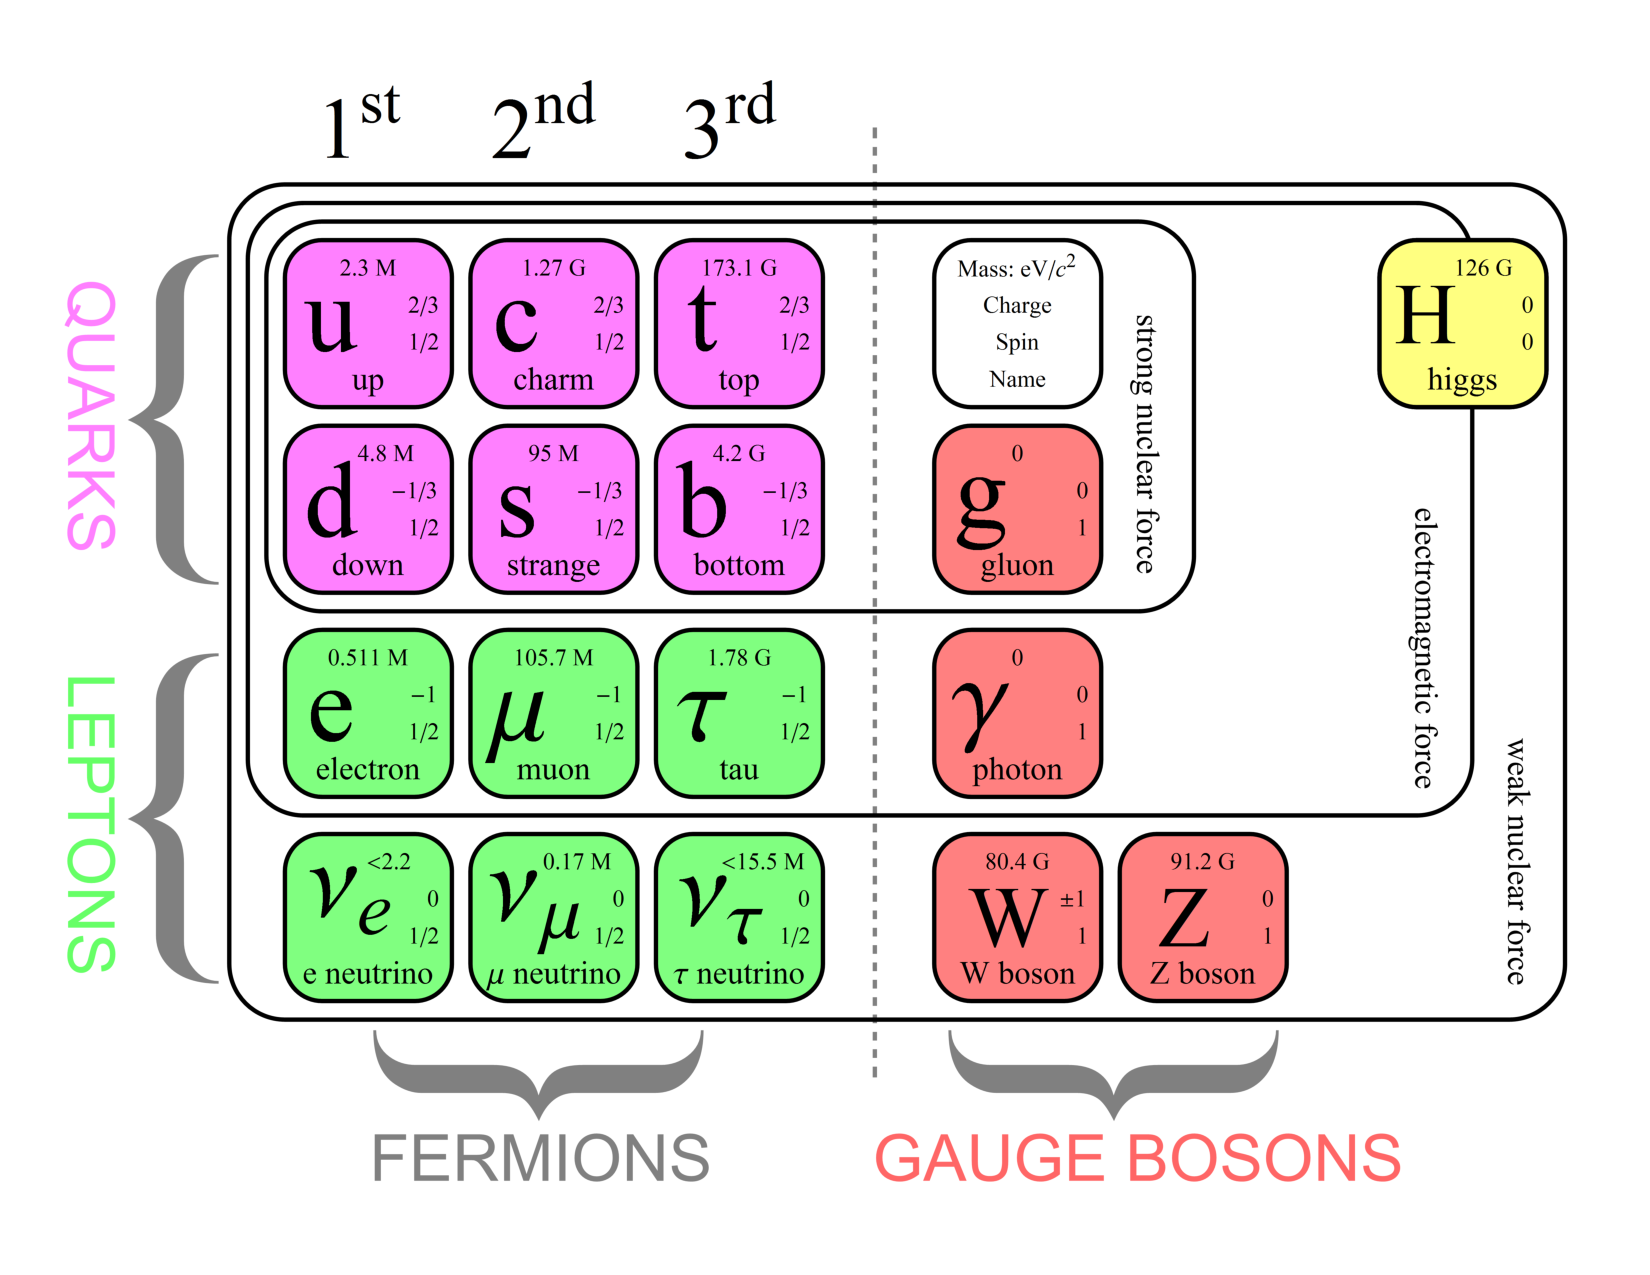
\includegraphics[width=0.7\textwidth]{introduction/plots/sm_particles.pdf}
     \caption{
The fundamental particles of the SM and some of their properties including their:
mass, electric charge, and spin. The units for mass are reported as electron volts divided by
the speed of light ($c$) squared and use scientific notation prefixes.
M for million, G for billion.
     }
     \label{fig:sm_particles}
\end{figure*}

The fermions can be further grouped into either quarks or leptons based on whether
they carry ``color'' charge or not. 
Quarks carry a color charge and have a fractional electric charge of either $-\frac{1}{3}e$ or $\frac{2}{3}e$
where $e$ is the elementary charge ($1.602 \times 10^{-19}$ Coulombs).
Where as the leptons are colorless (carry no color charge) and
have integer electric charge of 0$e$ or -1$e$. In Figure~\ref{fig:sm_particles} the fermions are
arranged according to what is called their mass ``generation'' with more massive
particles appearing to the right in the third mass generation column.

The first
mass generation column composes the fundamental particles which make up the ordinary matter
interact with every day. Up-quarks and down-quarks are the fundamental constituents within
protons and neutrons which build the atoms and molecules
making up the paper pages of this thesis or the metals and plastics in your computer. High energy protons
have a different composition and are discussed later in the thesis. Electrons are the
remaining fundamental particles we are familiar with and are also part of the basic 
structure of atoms. The electron neutrino is less familiar because it only
interacts with the other particles through the weak force and does not directly
contribute to the basic atoms.

The bosons are split into two groups, the gauge bosons which mediate the three fundamental
forces of the SM, and the solo Higgs boson which behaves differently
and will be discussed in the following chapter. 
The fundamental forces, their mediator particles, and the relative strength of that force
are listed in Table~\ref{tab:sm_forces}. The relatively weak strength of the gravitational
force is what allows the SM to still successfully predict the behavior
of particles despite not including the gravitational force.

\begin{table*}[htbp]
\centering
\begin{tabular}{lcc}
Fundamental Force        &    Force Mediator             & Relative Strength   \\
\hline
Strong                   &    gluon ($\Pg$)              &   1                 \\ 
Electromagnetic          &    photon ($\Pgg$)            &   $10^{-3}$         \\ 
Weak                     &    $\PW$ and $\PZ$ bosons     &   $10^{-14}$        \\ 
Gravitational            &    unknown                    &   $10^{-43}$        \\ 
\hline
\end{tabular}
\caption{
The fundamental forces, their mediator particles, and the relative strength of the force.
There has been no observed mediator for the gravitational force.
}
\label{tab:sm_forces}
\end{table*}

The strong force has the largest relative strength of the fundamental forces but
the reach, or distance over which the force can be felt, is very limited and is 
confined to the sub-atomic scale, $10^{-15}$m. The strong force is experienced
between particles with a color charge, exclusively gluons and quarks.
Figure~\ref{fig:sm_forces} shows a diagram of the SM particles with
lines linking force mediating bosons with the particles which experience that force.
For example, a line links the quarks with the gluons representing the
strong force.

The electromagnetic force follows after the strong force in order of largest relative
strength. The reach of the electromagnetic force is infinite and decreases with
distance as $\frac{1}{r^{2}}$. Despite its infinite reach, the electromagnetic 
force is not experienced on the macroscopic scale because stable matter is composed
of equal portions positively charged and negatively charged matter. This leads to
an overall neutral electrical charge for the universe. The electromagnetic force is experienced by all
electrically charged particles: quarks, the charged leptons, and the $\PW^{\pm}$ bosons.
This force is mediated by the photon which has neutral electric charged.
% XXX Add example of electrons holding you up in your chair, preventing you from
% falling through it?

The next force in descending order of relative strength is the weak force.
The weak force is experienced by
all of the leptons and the quarks and is mediated by the $\PW^{\pm}$ and $\PZ$ 
bosons. It is responsible for familiar phenomena such as the radioactive decay of atoms. 
Beta decay is one example of radioactive decay where, within an atomic nucleus,
a neutron is transformed into a proton and an electron and an electron antineutrino
(more on antiparticles following). Fundamentally, what happens
is the quark composition within the proton changes thereby changing the proton to a
neutron. This process is mediated by a $\PW^{-}$ boson which subsequently decays
to an electron and the antielectron neutrino.

The final and weakest force is the one we are most familiar with, the gravitational
force. Just like the electromagnetic force, the reach of the gravitational force 
is infinite and decreases with distance as $\frac{1}{r^{2}}$. Yet, unlike the
electromagnetic force, gravity is felt over extremely large distances. This is because
gravity is a purely attractive force which acts on all massive particles.
The force we are most colloquially familiar with is actually the
weakest of the four fundamental forces. Because the gravitational force is so weak
when talking about the effect on a single particle, it can be ignored for
all of the particle physics calculations throughout this thesis.

\begin{figure*}[htbp]
\centering
     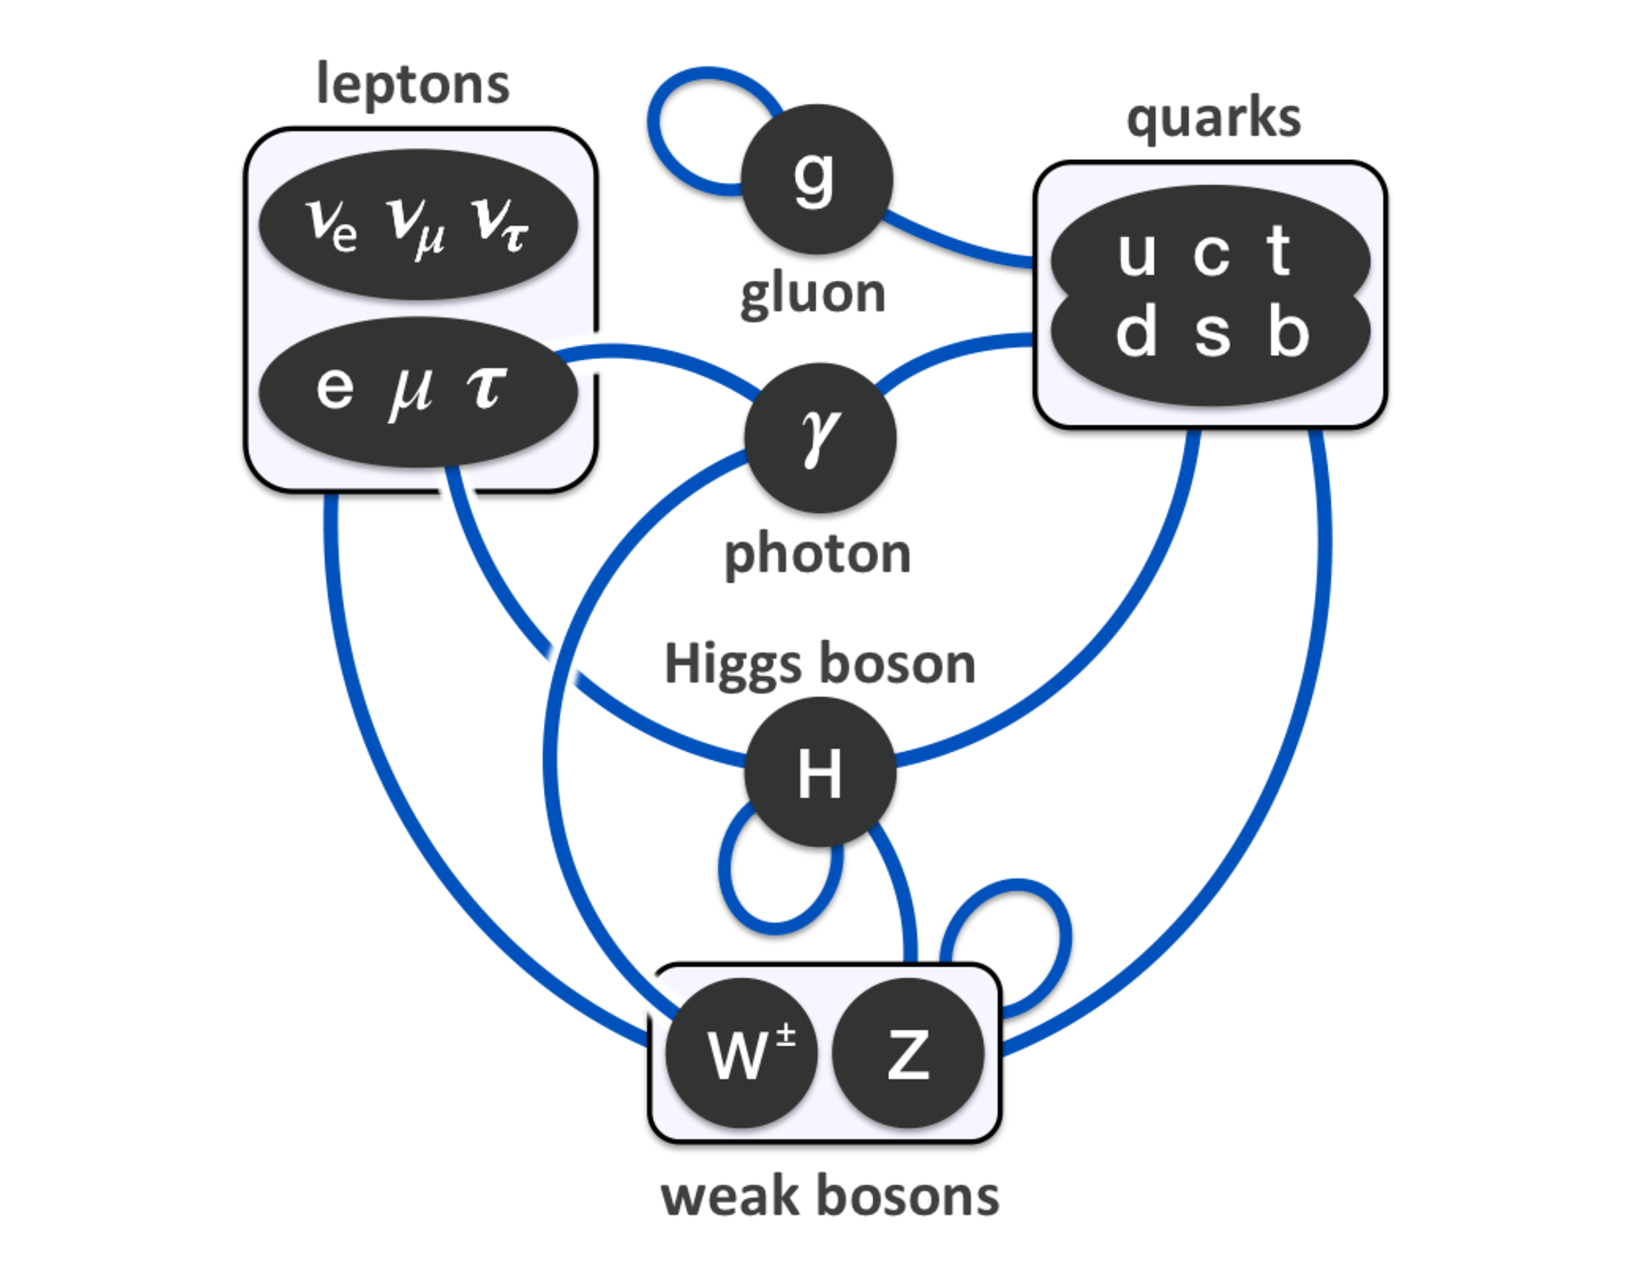
\includegraphics[width=0.7\textwidth]{introduction/plots/elementary_particle_interactions_SM.pdf}
     \caption{
Diagram showing the bosons arranged into a central column with the fermions in the
upper corners. The blue lines linking particles and groups of particles together
indicate that those fermions can be influenced by force associated to that mediator
boson. The Higgs boson in the center is discussed in Chapter~\ref{sec:pheno}.
     }
     \label{fig:sm_forces}
\end{figure*}

In addition to the particles shown in Figure~\ref{fig:sm_particles}, there exist antiparticles
which were mentioned previously in regard to beta decay.
Each SM particle has an antiparticle, though some particles, such as the photon
are their own antiparticle. Antiparticles have the same mass as their
``normal'' particle pair except they have opposite electric charge. The antiparticle
partner of the electron is the positron which is sometimes called an antielectron.
Antiparticles can be created in many types of interactions in particle physics experiments
and are relatively common. One characteristic of antiparticles is that when a particle and its 
corresponding antiparticle are in close proximity they can annihilate each other resulting in
a burst of energy.
Antiparticles are denoted in this thesis with a ``bar'' over the top of a particle symbol. For example
a top-quark is $t$ while an antitop-quark is $\bar{t}$.

For a more thorough treatment of the SM, its particles, and its forces see
Chapter~\ref{sec:pheno}.



\section{The Standard Model: Experimental Context}
The gap between the prediction of the Higgs boson and its discovery was a long 40 years.
Many of the particles making up the SM were not discovered when the Higgs boson
was originally being theorized. In fact, the existence of quarks or the discovery 
of gluons, the mediator of the strong force, were still to happen. The same is true
for the $\PW$ and the $\PZ$ bosons, the mediators of the weak force. The decades after the
1960s saw discovery after discovery, slowly piecing together and validating
the SM.

The internal structure of protons was illuminated by
deep inelastic scattering experiments carried out at SLAC which eventually led to 
the observation of the three least massive quarks: up ($u$), down ($d$), and strange ($s$)
in 1969~\cite{PhysRevLett.23.930,Breidenbach:1969kd}. In 1974, the $J/\Psi$ particle, a composite 
particle made from a charm quark ($c$) and a charm anti-quark ($\bar{c}$) was 
discovered~\cite{PhysRevLett.33.1404,PhysRevLett.33.1406}. 
The bottom quark ($b$) was discovered in 1977 via the decays of a new particle, the Upsilon
meson~\cite{PhysRevLett.39.252}. The top quark ($t$) was the last quark of the three
known generations discovered
and was not found until 1995 at Fermilab~\cite{PhysRevLett.74.2626,PhysRevLett.74.2632}.
The gluon which mediates the strong force for all of the quarks was discovered in 
1979 at DESY~\cite{PhysRevLett.43.830}.

Beyond the partons, physicists made discoveries of new bosons, specifically the mediators
of the weak force.
In 1983 the $\PW$ and the $\PZ$ bosons were discovered~\cite{AUBERT1983275,1983398}. 
These two bosons were the
most massive fundamental particles at the time of their discovery with masses of
84.4\GeV and 91.2\GeV, respectively.
A very important discovery laying the foundation for the analyses in this thesis is
the discovery of the third generation $\Pgt$ lepton, which was discovered
in 1975 by Martin Perl~\cite{PhysRevLett.35.1489}. While far from an exhaustive list,
these many discoveries give an indication of the strong background of experimental
research supporting the SM.

\section{Higgs Boson: Experimental Results}
As more pieces of the SM fell into place and particle accelerators became more powerful,
searches for the Higgs boson were conducted at multiple experiments such as the searches
at the LEP at CERN in the 1990s~\cite{Barate:2000ts,Abdallah:2003ip,Achard:2001pj,Abbiendi:2000ac}.
In the datasets corresponding to these searches, there were few enough potential Higgs
boson events that no discoveries could be made.
Instead, these searches all resulted in placing limits on the possible mass and cross section
of the Higgs boson. The Tevatron at Fermilab was active in Higgs boson searches through the early 2000s
with multiple analyses targeting the same decay process studied in this thesis, $\htt$. 
Similar to the LEP results, these analyses
placed limits on the possible mass and cross section of the Higgs boson~\cite{Aaltonen:2012jh, Abazov:2012zj}.

The discovery of the Higgs boson required higher collision energies than those provided
by the Tevatron, which reached a maximum center-of-mass collision energy of 1.96\TeV. The
LHC at CERN was designed to deliver this increase in collision energy and in 2010 the LHC started
delivering proton-proton collisions at up to 7\TeV; an increase to 8\TeV followed in 2012.
Using the proton-proton collision data with center-of-mass energy 7 and 8\TeV,
a particle compatible with the Higgs boson expectations was observed by the CMS and ATLAS experiments at the CERN LHC
in events where the Higgs boson decays to $\PZ\PZ$, $\Pgg\Pgg$, and 
$\PW\PW$~\cite{Aad:2012tfa, Chatrchyan:2012xdj, Chatrchyan:2013lba}.

Using this same set of data, other analysts pursued the $\htt$ decay process and
the CMS Collaboration showed evidence for the $\htt$ process with an observed
significance of 3.2 based on an expected significance of 3.7 standard deviations (s.d.)
for a Higgs boson mass of 125\GeV~\cite{Chatrchyan:2014nva}.
The ATLAS experiment reported evidence for the $\htt$ process 
with an observed (expected) significance of 4.5\,(3.4)
s.d. for a Higgs boson mass of 125\GeV~\cite{Aad:2015vsa}.
The combination of results from both experiments yields an observed (expected)
significance of 5.5\,(5.0) s.d.~\cite{Khachatryan:2016vau}.

Further analysis from both experiments, described in References~\cite{Aad:2015gba, Khachatryan:2014jba, 
Chatrchyan:2012jja, Aad:2013xqa, Khachatryan:2014kca,Sirunyan:2017exp},
established that the measured properties of the new particle,
including its spin, charge-parity properties, and coupling strengths to SM particles, 
are consistent with those expected for the Higgs boson predicted by the SM.
The mass of the Higgs boson has been determined to be
$125.09\pm0.21\stat\pm0.11\syst\GeV$, from a combination of
ATLAS and CMS measurements~\cite{Aad:2015zhl}. An example of these measurements
can be seen in Figure~\ref{fig:run_1_comb_mu} which shows the best fit value for the signal
strength for the Higgs boson production and decay processes. As can be seen, the
majority of the $\Pgt\Pgt$ decay process measurements shows agreement with the SM predictions for the Higgs
boson. The measurements corresponding to $\htt$ with the Higgs bosons produced in association
with a $\PW$ boson ($\PW\PH$) and the measurement of the Higgs boson produced with
two top-quarks ($\ttbar\PH$) show some deviation from the SM prediction. However, 
the uncertainties are sizable and are represented by the size of the 1$\sigma$ band. Further data collection and analysis
will reduce the size of the 1$\sigma$ uncertainty band and will show if 
these deviations are statistically significant or if they are 
temporary fluctuations that are smoothed out with more data collection.

\begin{figure*}[htbp]
\centering
     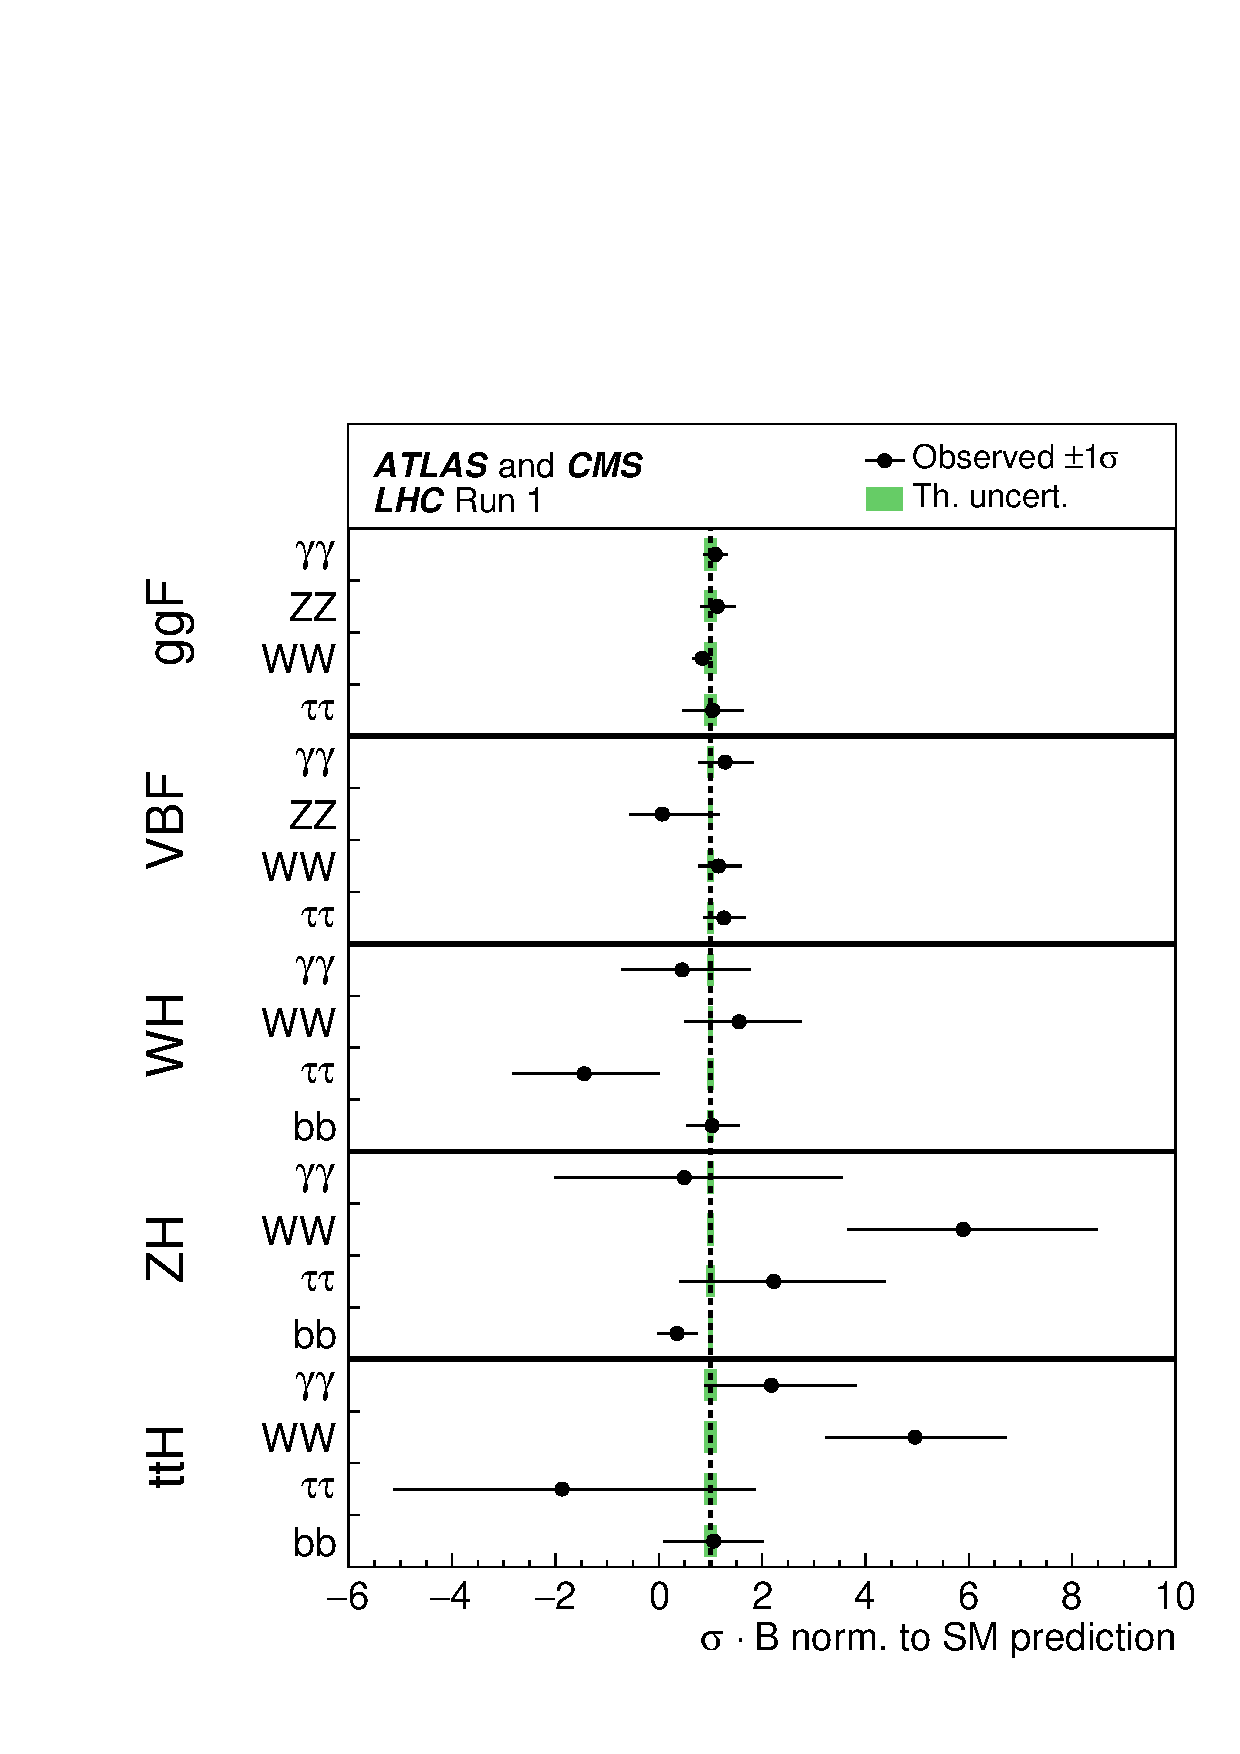
\includegraphics[width=0.6\textwidth]{introduction/plots/run_1_comb_mu.pdf}
     \caption{
The best fit values for the signal strength of the listed Higgs boson production
processes and decay processes. A value of 1 indicates perfect agreement with the SM.
The error bars indicate the 1$\sigma$ intervals. The green shaded bands indicate the
theoretical uncertainties in the predictions.
     }
     \label{fig:run_1_comb_mu}
\end{figure*}

This thesis builds on these previous experimental results at 7 and 8\TeV and measures the
properties of the Higgs boson in the $\htt$ decay process at 13\TeV center-of-mass 
collision energy. We establish the first 13\TeV observation of the $\htt$
process with an observed (expected) significance of 5.5\,(4.9) s.d. XXX FIX CITATION~\cite{HIG-18-007}. 
The best fit signal strengths are measured similar
to what is seen in Figure~\ref{fig:run_1_comb_mu}. Additionally, the couplings of the
Higgs boson to fermions and vector bosons is measured and is discussed in the final results
section of this thesis, Chapter~\ref{sec:cmb_results}.


%Wesley -
%One more point about the introduction. It should introduce your thesis topic.
%It should explain how your topics fit into or expand the standard model and
%how your topic(s) enhance our understanding beyond what preceded. You
%need to cover both the theoretical and experimental context (e.g. include
%a summary of the measurements that came before).
%
%Dasu - 
%As a hint, the intro should be accessible to non specialist. So, keep it simple, 
%written in English rather than CMSish. You should introduce SM as the most well 
%tested theory of nature at the fundamental level. The Higgs boson completes it.

